% !TeX spellcheck = cs_CZ
{\tikzset{external/prefix={tikz/FYZI/}}
 \tikzset{external/figure name/.add={ch29_}{}}
%=========================== Kapitola: Interference ===============================================
\chapter{Interference}\label{fyz:IchapXXIX}
\minitoc
  \section{Elektromagnetické vlny}\label{fyz:IchapXXIXsecI}
    V této kapitole si probereme matematicky důkladněji problematiku předcházející kapitoly. Pomocí 
    kvalitativních argumentů jsme si ukázali, že v radiačním poli dvou zdrojů jsou maxima a minima. 
    Nyní stojíme před problémem nejen kvalitativního, ale i detailního matematického popisu pole.
    
    \begin{figure}[ht!] %\ref{fyz:fig232}
      \centering
      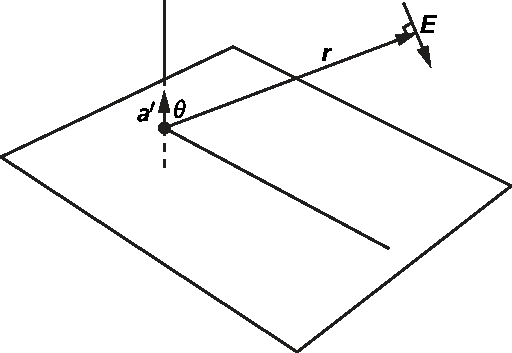
\includegraphics[width=0.7\linewidth]{fyz_fig232.pdf}
      \caption{Intenzita elektrického pole \(\vec{E}\) vyvolanéhokladným nábojem, jehož retardované 
               zrychlení je \(\vec{a'}\)
               (\cite[s.~379]{Feynman01})}
      \label{fyz:fig232}
    \end{figure}
    
    Již jsme provedli dosti uspokojivou fyzikální analýzu vztahu (\ref{fyz:eq301}), ale zůstává zde 
    několik  bodů týkajících se matematiky. V první řadě, pohybuje-li se náboj zrychleně podél 
    přímky nahoru a dolů s velmi malou amplitudou, intenzita pole v nějakém bodě ve směru 
    svírajícím s osou pohybu úhel \(\vartheta\) bude kolmá ke směru pohledu a leží v rovině, v níž 
    leží i zrychlení, i směr pohledu (obr. \ref{fyz:fig232}). Označíme-li vzdálenost \(r\), bude 
    mít intenzita elektrického pole v čase \(t\) velikost
    \begin{equation}\label{fyz:eq302}
      E(t) = -\frac{q}{4\pi\varepsilon_0c^2r}a\left(t-\frac{r}{c}\right)\sin\vartheta,
    \end{equation}
    kde \(a\left(t-\frac{r}{c}\right)\) je zrychlení v čase \(\left(t-\frac{r}{c}\right)\), tedy 
    retardované zrychlení.
    
    Bylo by zajímavé nakreslit obraz pole v různých situacích. Zajímavý je faktor \(a(t-r/c)\). 
    Abychom ho pochopili, vezměme si nejednodušší případ, kdy \(\vartheta=\ang{90}\) a pole 
    znázorněme graficky. Předtím jsme uvažovali, že se nacházíme najednom místě a ptáme se, jak se 
    v něm mění pole v závislosti na čase. Místo toho se nyní podíváme, jak pole vypadá v různých 
    místech prostoru v daném okamžiku. To, co chceme, je tedy „momentka“ znázorňující, jaké pole je 
    na různých místech. Samozřejmě, že to záleží na zrychlení náboje. Nejdříve předpokládejme, že 
    se náboj pohyboval určitým způsobem: zpočátku byl v klidu a najednou se začal nějak zrychlovat, 
    jak je ukázáno na obr. \ref{fyz:fig233} a pak se zastavil. Potom, o něco později, změříme 
    intenzitu pole na různých místech. Můžeme tvrdit, že pole bude mít tvar znázorněný na obr. 
    \ref{fyz:fig234}. V každém bodě je pole určeno zrychlením náboje v nějakém předcházejícím čase, 
    přičemž zpoždění je rovno \(r/c\). Pole ve vzdálenějších bodech je určeno zrychlením v 
    dřívějším a dřívějším čase. Takže křivka na obr. \ref{fyz:fig234} je v jistém smyslu 
    „obráceným“ průběhem zrychlení jako funkce času. Vzdálenost souvisí s časem prostřednictvím 
    konstantního škálovacího faktoru \(c\), který často uvažujeme rovný jedné. Snadno to můžeme 
    zjistit, podíváme-li se na matematické vlastnosti zrychlení a \((t-r/c)\). Když přidáme k \(t\) 
    malý čas \(\Delta t\), pro \(a(t - r/c)\) dostaneme stejnou hodnotu, jako kdybychom od \(r\) 
    odečítali malou vzdálenost: \(\Delta r = -c\Delta t\).
    
    \begin{figure}[ht!] %\ref{fyz:fig233}
      \centering
      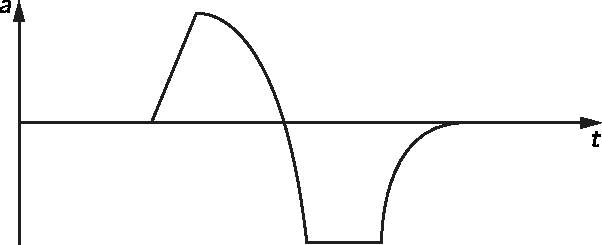
\includegraphics[width=0.7\linewidth]{fyz_fig233.pdf}
      \caption{Zrychlení náboje jako funkce času
               (\cite[s.~380]{Feynman01})}
      \label{fyz:fig233}
    \end{figure}

    \begin{figure}[ht!] %\ref{fyz:fig234}
      \centering
      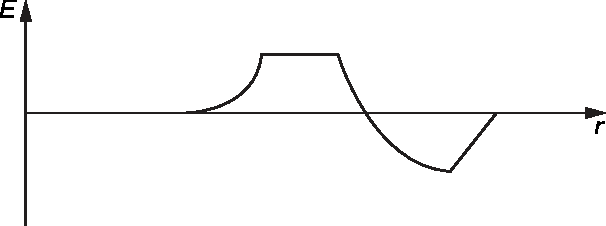
\includegraphics[width=0.7\linewidth]{fyz_fig234.pdf}
      \caption{Elektrické pole v pozdějším čase jako funkce polohy (změna \(1/r\) je zanedbána)
               (\cite[s.~380]{Feynman01})}
      \label{fyz:fig234}
    \end{figure}
    
    Vyjádřeno jinými slovy: Když přidáme malý čas \(\Delta t\), původní hodnotu \(a(t - r/c)\) 
    můžeme získat tak, že vzdálenost zvětšíme o \(\Delta r = c\Delta t\). To znamená, že s 
    rostoucím časem se pole pohybuje od zdroje jako vlna. To je důvod, proč někdy říkáme, že světlo 
    se šíří jako vlny. Je to ekvivalentní tomu, že pole se zpožduje nebo tomu, že elektrické pole 
    se s rostoucím časem šíří směrem ven do prostoru. 
    
    Zajímavým případem je, když se náboj \(q\) pohybuje nahoru a dolů jako oscilátor. Situace, 
    kterou jsme experimentálně studovali v předcházející kapitole byla taková, že posunutí \(x\) v 
    kterémkoli okamžiku bylo rovno určité konstantě \(x_0\) (amplitudě oscilací) násobené \(\cos 
    \omega t\), Zrychlení je pak
    \begin{equation}\label{fyz:eq303}
      a = -\omega^2x_0\cos\omega t = a_0\cos\omega t,
    \end{equation}
    kde \(a_0\) je maximální zrychlení \(-\omega^2x_0\). Dosazením do vztahu (\ref{fyz:eq302}) 
    najdeme

    \begin{equation}\label{fyz:eq304}
      E = -q\sin\vartheta\frac{a_0\cos\omega\left(t-\frac{r}{c}\right)}{4\pi\varepsilon_0rc^2}.
    \end{equation}
    
    Ponechme stranou úhel \(\vartheta\) i konstantní členy a podívejme se, jaká je funkce polohy a 
    času.
    
  \section{Energie záření}\label{fyz:IchapXXIXsecII}
    Nejdříve si uvědomme, že v kterémkoliv čase nebo na kterémkoliv místě se pole mění jako 
    převrácená hodnota vzdálenosti \(r\), jak jsme se zmínili již dříve. Nyní musíme upozornit, že 
    energetický obsah vlny nebo energetické účinky, jež může mít takové elektrické pole, jsou 
    úměrné druhé mocnině intenzity pole. Máme-li například nějaký náboj nebo oscilátor v 
    elektrickém poli a na tento oscilátor necháme působit pole, náboj se začne pohybovat. Je-li to 
    lineární oscilátor, zrychlení, rychlost a posunutí vyvolané působením elektrického pole na 
    tento náboj, budou všechny úměrné intenzitě pole. Proto kinetická energie, kterou získá náboj, 
    je úměrná druhé mocnině pole. Takže akceptujeme, že energie, kterou může pole dodat nějakému 
    systému, je nějak úměrná druhé mocnině intenzity pole.

    \begin{figure}[ht!] %\ref{fyz:fig235}
      \centering
      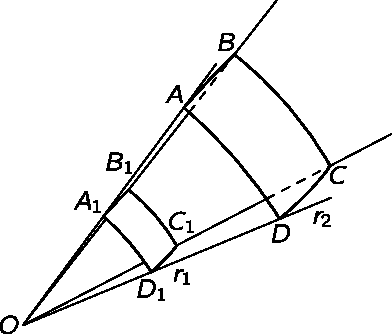
\includegraphics[width=0.5\linewidth]{fyz_fig235.pdf}
      \caption{Energie proudící v jehlanu \(OABCD\) nezávisi na vzdálenosti \(r\)
               (\cite[s.~381]{Feynman01})}
      \label{fyz:fig235}
    \end{figure}
    
    To znamená, že energie, kterou může zdroj dodat, se bude při vzdalování stále zmenšovat 
    Skutečně, mění se nepřímo úměrně druhé mocnině vzdálenosti; ale to lze velmi snadno vysvětlit. 
    Kdybychom chtěli zachytit všechnu energii vlny v nějakém kuželi ve vzdálenosti \(r\) (obr. 
    \ref{fyz:fig235}) a totéž bychom udělali ve vzdálenosti, zjistili bychom, že množství energie 
    připadající na jednotkovou plochu v jakémkoliv místě závisí nepřímo úměrně na druhé mocnině 
    \(r\), ale velikost plochy protínající kužel závisí přímo úměrně na druhé mocnině \(r\). Takže 
    energie, kterou můžeme získat z vlny v nějakém daném prostorovém úhlu, je stále stejná, bez 
    ohledu na to, jak jsme daleko! Konkrétně, celková energie, již bychom mohli získat z celé vlny 
    tím, že bychom dokola umístili absorbující oscilátory, představuje určitou neměnnou hodnotu. 
    Proto skutečnost, že amplituda \(E\) se mění jako \(1/r\), představuje totéž, jako kdybychom 
    řekli, že existuje tok energie, jenž se neztrácí, stále proudí a rozšiřuje se na stále větší a 
    větší oblast. Tím, že náboj osciloval, ztratil určitou energii, jíž nemůže nikdy znova nabýt, 
    energie se neustále šíří dál a dál, aniž by se nějak zmenšovala. Tedy, jsme-li dostatečně 
    vzdáleni tak, aby naše základní aproximace byla dostatečně dobrá, náboj nemůže získat zpět 
    energii,jež byla vyzářena, Samozřejmě, tato energie stále někde existuje a lze ji zachytit 
    pomocí jiných systémů. Tuto „ztrátu“ energie budeme studovat dále ve kapitole 
    \ref{fyz:IchapXXXII}.
    
    Nyní se pojďme podrobněji zabývat tím, jak se mění vlna (\ref{fyz:eq304}) jako funkce času v 
    daném místě a jako funkce polohy v daném čase. Opět zanedbáme závislost na \(1/r\) a konstantě.
    
  \section{Sinusoidální vlny}\label{fyz:IchapXXIXsecIII}
    Nejdříve zafixujeme polohu \(r\) a sledujme pole jako funkci času. Pole osciluje s úlohovou 
    frekvencí \(\omega\). \textbf{Úhlovou frekvenci} \(\omega\) lze definovat jako \emph{rychlost 
    změny fáze s časem} (radiány za sekundu). Něco takového jsme již studovali, proto by nám měla 
    být problematika dost známá. Vypočítali jsme, čemu je rovna \emph{perioda} - to je doba 
    potřebná k jedné oscilaci, jednomu úplnému cyklu. Je rovna \(2\pi/\omega\), neboť \(\omega\) 
    násobené periodou je rovna jednomu cyklu funkce kosinus.
    
    Nyní si zavedeme novou veličinu, která se ve fyzice často používá. Souvisí s opačnou situací, 
    kdy \(t\) zafixujeme a na vlnu se díváme jako na funkci vzdálenosti \(r\). Vidíme, že vlna jako 
    funkce \(r\) (\ref{fyz:eq304}) také osciluje. Odhlédneme-li od závislosti \(1/r\), vidíme, že 
    \(E\) osciluje se změnou polohy. Takže analogicky s \(\omega\) můžeme definovat veličinu 
    nazvanou \textbf{vlnové číslo} a označenou jako \(k\). Je definována jako \emph{rychlost změny 
    fáze se vzdáleností} (radiány na metr). Fáze se tedy mění, pohybujeme-li se v prostoru, při 
    neměnném čase.
    
    Existuje další veličina, jež odpovídá periodě a již bychom mohli nazvat periodou v prostoru, 
    ale obvykle se nazývá \textbf{vlnová délka} a označuje se \(\lambda\). Vlnová délka představuje 
    \emph{vzdálenost, na níž se rozprostírá jeden úplný cyklus}. Pak lze snadno vidět, že vlnová 
    délka je rovna \(2\pi/k\), protože \(k\) násobené vlnovou délkou je rovna počtu radiánů, o něž 
    se změnila fáze (když je to součin změny radiánů na metr a počtu metrů) a projeden cyklus musí 
    být rovna \(2\pi\). Takže \(k\lambda=2\pi\) je analogie vztahu \(\omega T= 2\pi\).
    
    Pro naši konkrétní vlnu platil mezi frekvencí a vlnovou délkou určitý vztah, ale uvedené 
    definice \(k\) a \(\omega\) platí zcela obecně a za jiných fyzikálních podmínek mezi vlnovou 
    délkou a frekvencí může být jiná souvislost. Avšak v našem případě lze snadno určit rychlost 
    změny fáze se vzdáleností, neboť, když označíme fázi \(\varphi=\omega(t-r/c)\) a vyjádříme její 
    parciální derivaci podle \(r\), pro rychlost změny \(\pder{\varphi}{r}\) platí
    
    \begin{equation}\label{fyz:eq305}
      \abs{\pder{\varphi}{r}} = k = \frac{\omega}{c}.
    \end{equation}
    
    Existuje více způsobů, jak vyjádřit tento vztah. Například
    \begin{subequations}\label{fyz:eq306}
      \begin{align}
        \lambda        &= cT      \label{fyz:eq306a}  \\
        \omega         &= ck      \label{fyz:eq306b}  \\
        \lambda f      &= c       \label{fyz:eq306c}  \\
        \omega\lambda  &= 2\pi c  \label{fyz:eq306d}  
      \end{align}
    \end{subequations}
    
    Proč je vlnová délka rovna součinu \(c\) a periody? To je velmi snadné - protože, když sedíme 
    nehybně a čekáme, až kolem nás proběhne jedna perioda, přesunou se vlny šířící se rychlostí 
    \(c\) o vzdálenost \(cT\) a samozřejmě projdou právě jednu vlnovou délku.
    
    Za jiné fyzikální situace odlišné od případu světla nemusí \(k\) tak jednoduše souviset s 
    \(\omega\). Označíme-li vzdálenost podél osy \(x\), vztah pro kosinovou vlnu s vlnovým číslem 
    \(k\) a úhlovou frekvencí \(\omega\) šířící se ve směru \(x\) se zapíše obecně jako 
    \(\cos(\omega t-kx)\).
    
    Když jsme si určili pojem vlnové délky, můžeme si říct něco o podmínkách, za kterých platí 
    (\ref{fyz:eq304}). Vzpomínáme si, že pole se skládá z více složek; jedna z nich se mění jako 
    \(1/r\), druhá jako \(1/r^2\) a jiné dokonce rychleji. Stálo by za to zjistit, zajakých 
    okolností je složka pole \(1/r\) nejdůležitější a ostatní poměrně malé. Přirozenou odpovědí je: 
    Jdeme-li dostatečně daleko, neboť členy, jež se mění nepřímo úměrně druhé mocnině, se 
    nevyhnutně stávají zanedbatelnými v porovnání s členem \(1/r\). Jak daleko je „dostatečně 
    daleko“? Kvalitativně řečeno je to tak daleko, že ostatní členy jsou řádově o \(\lambda/r\) 
    menší než člen \(1/r\). Jakmile jsme dále než je vzdálenost několika vlnových délek, je 
    (\ref{fyz:eq304}) pro pole vynikající aproximací. Někdy se oblast za vzdáleností několika 
    vlnových délek nazývá \emph{„vlnová zóna“}.
    
  \section{Dva dipólové zářiče}\label{fyz:IchapXXIXsecIV}
    Dále se věnujme matematice, která se týká skládání účinků od dvou oscilátorů při hledání 
    výsledného pole v daném bodě. V několika případech, o nichž jsme již uvažovali v předcházející 
    kapitole, je to velmi snadné. Nejdříve provedeme kvalitativní a později více kvantitativní 
    popis. Vezměme si jednoduchý případ, kdy jsou středy oscilátorů umístěny ve stejné horizontální 
    rovině jako detektor a směr vibrací je vertikální.

    \begin{figure}[ht!]      %\ref{fyz:fig236}
      \centering
      \begin{tabular}{cc}
        \subfloat[ ]{\label{fyz:fig236a}
          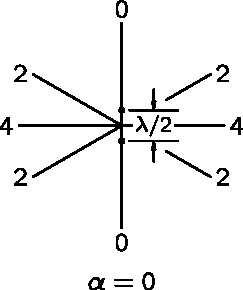
\includegraphics[width=0.4\linewidth]{fyz_fig236a.pdf}}
        \hspace{-1em}                                                       &
        \subfloat[ ]{\label{fyz:fig236b}
          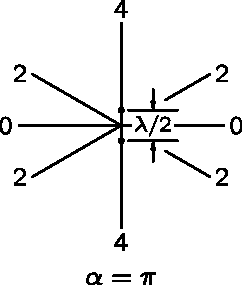
\includegraphics[width=0.4\linewidth]{fyz_fig236b.pdf}}
      \end{tabular}
      \caption{Intenzita pole v různých směrech od dvou dipólových oscilátorů vzdálených od sebe  o 
               polovinu vlnové délky. Vlevo:ve fázi, když \(\alpha = 0\).Vpravo: v protifázi, když 
               \(\alpha = \pi\) \cite[s.~383]{Feynman01}}
      \label{fyz:fig236}
    \end{figure}

    Na obr. \ref{fyz:fig236a} je pohled shora na takové dva oscilátory a v tomto konkrétním případě 
    jsou od sebe vzdáleny o polovinu vlnové délky ve směru sever-jih. Oscilují současně se stejnou 
    fází, již nazveme nulovou. Rádi bychom našli intenzitu záření v různých směrech. Intenzitou 
    záření rozumíme množství energie nesené polem za sekundu, úměrné druhé mocnině časové střední 
    hodnoty intenzity elektrického pole. Takže to, co máme hledat, chceme-li vědět, jak je světlo 
    jasné, je druhá mocnina intenzity elektrického pole, nikoli samotná intenzita pole. Intenzita 
    elektrického pole nám udává velikost síly působící na stacionární náboj, ale množství energie 
    letící za sekundu kolem (ve wattech na čtvereční metr) je úměrné druhé mocnině intenzity 
    elektrického pole. Konstantu úměrnosti odvodíme v další kapitole. Při pohledu ze západní strany 
    přispívají oba oscilátory stejně a ve fázi, takže elektrické pole je dvakrát tak silné než by 
    bylo, kdyby tam byl jen jeden oscilátor. Proto intenzita záření je čtyřikrát silnější než by 
    byla, kdyby tam byl jen jeden oscilátor (Čísla na obr. \ref{fyz:fig236} znázorňují, jaká bude 
    intenzita pole v porovnání s tím, že by tam byl jen jeden oscilátor s jednotkovou silou.) Při 
    pozorování ze severní nebo jižní strany je účinek jednoho oscilátoru fázově posunut vzhledem k 
    účinku druhého oscilátoru přesně o půl kmitu, neboť jsou od sebe vzdáleny o polovinu vlnové 
    délky, a jejich pole navzájem ruší. Pod určitým úhlem (přesně \ang{30}) je intenzita rovna 
    \(2\), takže intenzita klesá jako \(4\), \(2\), \(0\) atd. Potřebujeme se naučit, jak tato 
    čísla najít pro jiné úhly. Je to otázka skládání dvou oscilací s různými fázemi.
    
    Podívejme se zběžně na některé jiné zajímavé případy. Opět předpokládejme, že oscilátory jsou 
    vzdáleny o polovinu vlnové délky, ale fáze \(\alpha\) jednoho se opožduje o půl periody za fází 
    druhého (obr. \ref{fyz:fig236b}). Intenzita v západním směru je nyní rovna nule, neboť jeden 
    oscilátor„tlačí“, když druhý „tahá“. V severním směru přichází signál od bližšího oscilátoru za 
    určitý čas a od druhého o půlperiody později. Ten však byl původně o půl periody posunut, je 
    proto nyní přesně v časovém souladu s prvním a intenzita v tomto směruje rovna \(4\) jednotkám. 
    Intenzita ve směru pod úhlem \ang{30} je stále rovna \(2\), jak dále uvidíme. Dostáváme se k 
    zajímavému případu, jenž se vyznačuje užitečnými vlastnostmi. Poznamenejme, že jeden z důvodů, 
    proč jsou tyto souvislosti mezi oscilátory zajímavé,je směrování radiových vysílačů. Například, 
    když stavíme anténový systém a chceme vysílat signál, řekněme na Havaj, sestavíme antény, jako 
    na obr. \ref{fyz:fig236a}, a vysíláme s našimi dvěma anténami ve fázi, neboť Havaj se od nás 
    nachází na západ. Potom se rozhodneme, že zítra budeme vysílat směrem do Alberty v Kanadě. 
    Protože je od nás na sever a ne na západ, jediné, co stačí udělat, je obrátit fázi jedné z 
    našich anténa můžeme vysílat na sever. Anténové systémy můžeme sestavit různě. Náš systém je 
    ten nejednodušší možný. Můžeme však sestavit mnohem složitější systémy. Změnou fáze v různých 
    anténách můžeme paprsky směřovat do různých směrů a největší výkon vysílat v žádaném směru aniž 
    bychom s anténou pohnulil V obou předcházejících případech ztrácíme mnoho výkonu unikajícího na 
    opačnou stranu. Při vysílání směrem k Albertě jde stejný výkon i na Velikonoční ostrov, a bylo 
    by zajímavé si položit otázku, zda by bylo možné vysílat jen jedním směrem. Na první pohled se 
    nám může zdát, že s takovým párem antén bude výsledek vždy symetrický. Abychom ukázali i 
    takovou možnost, podívejme se na případ, jenž není symetrický. Co se stane, budou-li antény od 
    sebe vzdáleny o čtvrtvlnové délky a když ta, která je severněji (\(S\)), se bude zpožďovat o 
    čtvrt periody za tou, která je jižněji (\(J\))? (Obr. \ref{fyz:fig237}) V západním směru, jak 
    později uvidíme, dostaneme \(2\). V jižním směru dostaneme nulu, neboť signál z \(J\) přijde za 
    určitý čas, ale signál z \(S\) přijde o čtvrt periody později, ale protože je sám o čtvrt 
    periody opožděn, bude výsledné zpoždění rovno půl periodě a výsledný efekt bude nulový. Na 
    druhé straně, v severním směru přichází signál o čtvrt periody dříve než z \(J\), neboť je blíž 
    o čtvrt vlnové délky, avšak jeho fáze se opožďuje o čtvrt periody, což se právě kompenzuje s 
    časovým zpožděním, tak že oba signály jsou ve fázi, intenzita pole je dvakrát tak velká a 
    energie čtyřikrát tak velká.

    \begin{figure}[ht!] %\ref{fyz:fig237}
      \centering
      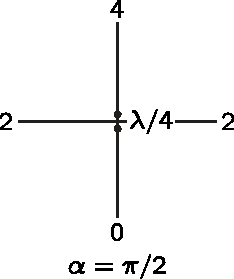
\includegraphics[width=0.4\linewidth]{fyz_fig237.pdf}
      \caption{Pár dipólových antén vyzařující maximální výkon vj ednom směru
               (\cite[s.~384]{Feynman01})}
      \label{fyz:fig237}
    \end{figure}
    
    Pomocí určité šikovnosti při rozmisťování anténa při nastavení jejich fází tedy můžeme vyslat 
    celý výkon v jednom směru. Energie je však ještě stále rozložena ve velkém prostorovém úhlu. 
    Můžeme zařídit, aby výkon byl ostřeji nasměrován v jednom směru? Opět vezměme případ vysílání 
    na Havaj, kde vysíláme vlny na západ a na východ, přičemž se šíří v dost velkém úhlu, neboť 
    dokonce při \ang{30} máme stále poloviční intenzitu - zbytečně ztrácíme výkon. Můžeme udělat 
    něco lepšího? Mějme situaci, v níž je vzdálenost mezi anténami rovna deseti vlnovým délkám 
    (obr. \ref{fyz:fig238}), což je víc podobné naší experimentální situaci z předešlé kapitoly s 
    rozestupem antén rovnajícím se několika vlnovým délkám a ne malému zlomku vlnové délky. Zde 
    máme zcela jiný obraz.
    
    \begin{figure}[ht!] %\ref{fyz:fig238}
      \centering
      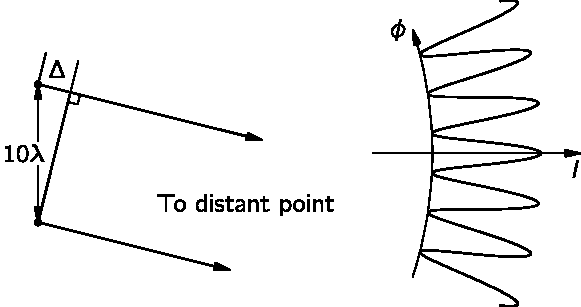
\includegraphics[width=0.7\linewidth]{fyz_fig238.pdf}
      \caption{ Obraz rozložení intenzity pro dva dipóly vzdálené od sebe o \(10\lambda\)
               (\cite[s.~385]{Feynman01})}
      \label{fyz:fig238}
    \end{figure}
    
    Je-li rozestup mezi anténami roven deseti vlnovým délkám (pro jednoduchost bereme případ se 
    stejnými fázemi), ve směru východ-západ jsou antény ve fázi a dostáváme velkou intenzitu, 
    čtyřikrát větší než bychom měli pouze při jedné anténě. Na druhé straně, při směru odlišném jen 
    o velmi malý úhel, odpovídají rozdíly v časech polovině periody a intenzita je rovna nule. 
    Přesněji, když vyznačíme směr od každého z oscilátorů do vzdáleného bodu a když je rozdíl 
    \(\Delta\) těchto dvou vzdáleností roven \(\lambda/2\) (polovina kmitu), budou kmity v 
    protifázi a vyskytne se první nula. (Části obrázku nejsou nakresleny ve stejném měřítku, je to 
    jen hrubý náčrt.) To znamená, že v žádaném směru máme velmi ostrý paprsek, neboť, když se jen o 
    málo odchýlíme, ztratíme celou intenzitu. Bohužel, pro praktické účely konstrukce vysílacích 
    soustav, zdvojnásobí-li se vzdálenost \(\Delta\), posunou se fáze o celou periodu, což je 
    přesně totéž, jako kdyby byly znovu ve fázi! Takže máme mnoho po sobě jdoucích maxim a minim, 
    podobných těm, jež jsme našli v kapitole \ref{fyz:IchapXXVIII} při vzdálenosti antén rovnajícím 
    se dvěma půlvlnovým délkám.
    
   \begin{figure}[ht!] %\ref{fyz:fig239}
      \centering
      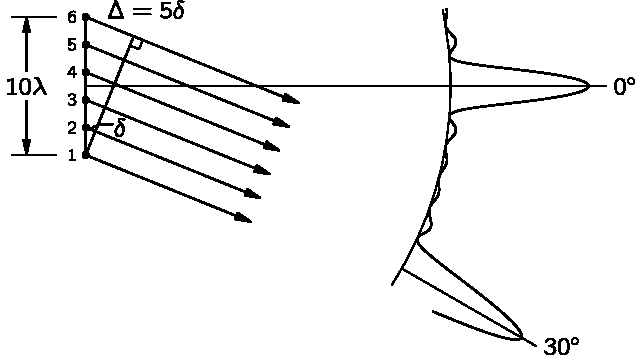
\includegraphics[width=0.7\linewidth]{fyz_fig239.pdf}
      \caption{Šestidipólová anténová souprava a část rozložení její intenzity. 
               (\cite[s.~385]{Feynman01})}
      \label{fyz:fig239}
    \end{figure}
    
    Jak se můžeme zbavit všech těchto nadbytečných maxim nebo, jak se jim říká, \emph{„laloků“}? 
    Můžeme se jich zbavit velmi zajímavým způsobem. Předpokládejme, že bychom mezi dvě antény 
    umístili další sadu antén, takže vnější by byly stále vzdáleny o \(10\lambda\), ale mezi ně 
    bychom, řekněme ve vzdálenosti každé \(2\lambda\), umístili další anténu všechny ve fázi. Nyní 
    budeme mít šest antén a je samozřejmé, že ve směru východ-západ bude intenzita mnohem větší než 
    při jedné anténě. Intenzita pole bude šestkrát větší a intenzita záření třicet šestkrát větší 
    (rovna druhé mocnině intenzity pole). V tomto směru budeme mít \(36\) jednotek. Podíváme-li se 
    nyní na okolní body, nulu opět najdeme přibližně jako předtím, ale jdeme-li dál, tam, kde jsme 
    měli velký „hrb“, najdeme nyní „hrb“ mnohem menší. Pokusme se ukázat proč.
    
    Důvod je třeba hledat v tom, že při vzdálenosti \(\Delta\) rovnající se vlnové délce bychom 
    sice mohli očekávat „hrb“, neboť dipóly \(1\) a \(6\) jsou tehdy ve fázi a vzájemně se 
    podporují při vytváření pole v tomto směru, ale dipóly \(3\) a \(4\) jsou přibližně o půl vlny 
    fázově posunuty vzhledem k \(1\) a \(6\), a i když \(1\) a \(6\) pracují spolu, \(3\) a \(4\) 
    také pracují spolu, ale s opačnou fází. Proto je intenzita v tomto směru velmi malá, ale 
    nenulová, protože účinky se úplně neruší. Takový jev nastává při ostatních maximech - dostáváme 
    velmi malé „hrby“, přičemž paprsek je v žádaném směru velmi silný. V tomto konkrétním případě 
    nastane i něco jiného - jsou-li vzdálenosti mezi sousedními dipóly \(2\lambda\), lze najít 
    takový úhel, při kterém jsou rozdíly vzdálenosti do \(\delta\) sousedních dipólů rovny přesně 
    jedné vlnové délce, takže účinky všech dipólů jsou opět ve fázi. Fáze každého dipólu je 
    vzhledem k následující fázi posunuta o celý cyklus, takže všechny jsou opět ve fázi a v tomto 
    směru máme další silný paprsek! V praxi je možné se tomu vyhnout, neboť dipóly se k sobě mohou 
    přiblížit těsněji než je vzdálenost jedné vlnové délky. Přidáme-li další antény s rozestupem 
    menším než jedna vlnová délka, nemůže takové maximum vzniknout. Avšak fakt, že při určitých 
    úhlech vzniknout může jsou-li vzdálenosti mezi anténami větší než jedna vlnová délka, je velmi 
    zajímavý a je to užitečný jev pro jiné aplikace - nikoli pro šíření rádiových vln, ale pro 
    \emph{difrakční mřížky}.
    
  \section{Matematika interference}\label{fyz:IchapXXIXsecV}
    Skončili jsme kvalitativní rozbor jevů souvisejících s dipólovými zářiči a je třeba se naučit, 
    jak je analyzovat kvantitativně. Chceme-li najít účinek od dvou zdrojů pod nějakým úhlem v 
    nejobecnějším případě, když mezi oscilátory je nějaký vzájemný fázový posun a a amplitudy 
    \(A_1\) a \(A_2\), nejsou stejné, zjistíme, že musíme sčítat dva kosiny se stejnými 
    frekvencemi, ale s rozdílnými fázemi. Tento rozdíl fází lze snadno najít; skládá se ze zpoždění 
    způsobeného rozdílem vzdáleností a vlastním, zabudovaným, fázovým posunem oscilátorů. 
    Matematicky musíme najít součet \(R\) dvou vln: \(R = A_1\cos(\omega t + \varphi_1) + 
    A_2\cos(\omega t + \varphi_2)\). Jak se to dělá? 
    
    Je to skutečně velmi snadné a předpokládáme, že to už umíme udělat. Přesto však naznačíme, jak 
    se to dělá. Ovládáme-li dobře matematiku a dost toho víme o kosinu a sinu, můžeme to snadno 
    vypočítat přímo. Nejjednodušší případ je, když \(A_1\) a \(A_2\), jsou stejné, řekněme, že jsou 
    obě rovny \(A\). V takovém případě (takovou metodu můžeme nazvat \emph{trigonometrickou metodou 
    řešení}) máme
    \begin{equation}\label{fyz:eq311}
      R = A\left[\cos(\omega t + \varphi_1) + \cos(\omega t + \varphi_2)\right]. 
    \end{equation}
    Na hodinách trigonometrie jsme se snad naučili pravidlo
    \begin{equation}\label{fyz:eq309}
      \cos A + \cos B =2\cos\frac{1}{2}(A + B)\cos\frac{1}{2}(A - B)
    \end{equation}
    Známe-li ho, můžeme ihned napsat
    \begin{equation}\label{fyz:eq310}
      R = 2A\cos\frac{1}{2}(\varphi_1 - \varphi_2)
            \cos\left(\omega t + \frac{1}{2}\varphi_1 + \frac{1}{2}\varphi_2\right)
    \end{equation}
    vidíme tedy, že máme řešení ve tvaru vlny s novou fází a s novou amplitudou. Obecně je 
    výsledkem vlna s novou amplitudou \(A_R\) (můžeme ji nazvat výslednou amplitudou), oscilující 
    se stejnou frekvencí, ale s různou fází \(\varphi_R\) nazvanou výsledná fáze. V našem 
    konkrétním případě jevysledná amplituda
    \begin{equation}\label{fyz:eq312}
      A_R = 2A\cos\frac{1}{2}(\varphi_1 - \varphi_2)
    \end{equation}
    a výsledná fáze je rovna průměru z obou fází. Náš problém je vyřešen.
    
    Nyní předpokládejme, že si nepamatujeme, že součet dvou kosinů je roven dvojnásobku součinu 
    kosinů polovičního součtu a kosinu polovičního rozdílu. Pak můžeme použít jiný způsob analýzy, 
    jenž je víc geometrický. Každou funkci kosinus \(\omega t\) si můžeme představit jako 
    horizontální projekci rotujícího vektoru. Předpokládejme, že vektor \(\vec{A}_1\), délky 
    \(A_1\), rotuje v čase, takže úhel, který svírá s horizontální osou je \(\omega t + 
    \varphi_1\). Na chvíli vynecháme \(\omega t\) a uvidíme, že se nic nestane. Předpokládejme, že 
    v čase \(t=0\) uděláme momentku, i když ve skutečnosti obraz rotuje s úhlovou rychlostí 
    \(\omega\) (obr. \ref{fyz:fig240}). Průmět \(\vec{A}_1\), na horizontální osuje přesně 
    \(A_1\cos(\omega t + \varphi_1)\). Nyní, pro \(t = 0\), můžeme znázornit druhou vlnu jako 
    nějaký jiný, také rotující vektor \(\vec{A}_2\), délky \(A_2\), a pod úhlem \(\varphi_2\). Oba 
    vektory rotují se stejnou úhlovou rychlostí, proto se jejich vzájemná poloha nemění. Systém se 
    otáčí jako tuhé těleso. Horizontální průmět \(\vec{A}_2\) je \(A_2\cos(\omega t + \varphi_2)\). 
    Z vektorového počtu však víme, že sčítáme-li dva vektory (pomocí běžného pravidla rovnoběžníka) 
    a nakreslíme výsledný vektor \(\vec{A}_R\), \(x\)-ová složka výslednice je rovna součtu 
    \(x\)-ových složek jednotlivých vektorů. To je řešení našeho problému. Snadno se můžeme 
    přesvědčit, že pro speciální případ \(A_1 = A_2 = A\), jímž jsme se již zabývali, dostaneme 
    správný výsledek. Z obr. \ref{fyz:fig240} vidíme, že v tomto případě leží \(\vec{A}_R\) 
    uprostřed mezi \(\vec{A}_1\) a \(\vec{A}_2\) a s každým z nich svírá úhel \(1/2(\varphi_2 - 
    \varphi_1)\). Proto vidíme, že jako předtím \(A_R = 2A\cos\frac{1}{2}(\varphi_2 - \varphi_1)\). 
    Z trojúhelníku je také zřejmé, že otáčí-li se \(\vec{A}_R\) dokola, jeho fáze je rovna průměru 
    úhlů příslušejících \(\vec{A}_1\) a \(\vec{A}_2\), v případě, že amplitudy jsou stejné. Je
    jasné, že stejně jednoduše můžeme najít řešení i pro případ, kdy amplitudy nejsou stejné. To 
    můžeme nazvat geometrickým způsobem řešení problému.
    
    \begin{figure}[ht!] %\ref{fyz:fig240}
      \centering
      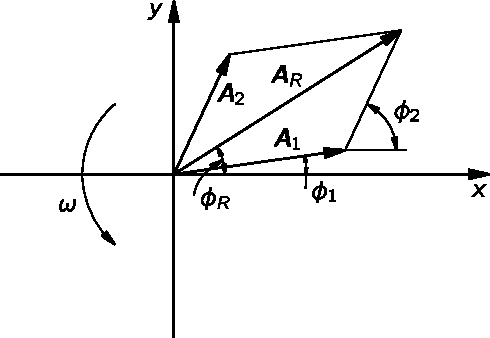
\includegraphics[width=0.8\linewidth]{fyz_fig240.pdf}
      \caption{Geometrický způsob skládání dvou kosinových vln. Celý diagram rotuje proti směru 
               hodinových ručiček úhlovou rychlostí \(\omega\).
               (\cite[s.~387]{Feynman01})}
      \label{fyz:fig240}
    \end{figure}
    
    Existuje ještě další způsob řešení tohoto problému a to analytický. Znamená tolik, že místo 
    toho, abychom museli kreslit obrázky (jako obr. \ref{fyz:fig240}), můžeme napsat něco, co říká 
    totéž co obrázek: místo kreslení vektorů píšeme komplexní čísla jako reprezentaci vektorů. 
    Reálné části komplexních čísel jsou skutečné fyzikální veličiny. V našem případě mohou být vlny 
    zapsány takto: \(A_1\exp{i(\omega t + \varphi_1)}\) (reálná částje \(A_1\cos(\omega t + 
    \varphi_1)\)) a \(A_2\exp{i(\omega t + \varphi_2)}\). Nyní je můžeme sčítat
    \begin{align}
      R &= A_1e^{i(\omega t + \varphi_1)} + A_2e^{i(\omega t + \varphi_2)} \nonumber       \\
        &= \left(A_1e^{i\varphi_1} + A_2e^{i\varphi_2}\right)e^{i\omega t} \label{fyz:eq308}
     \shortintertext{nebo pro komplexní amplitudu}
     \hat{R} &= A_1e^{i\varphi_1} + A_2e^{i\varphi_2} = A_Re^{i\varphi_R}
    \end{align}    
    To je řešení daného problému, neboť výsledek má tvar komplexního čísla s velikostí \(A_R\). a 
    fází \(\varphi_R\).
    
    Abychom viděli, jak se tato metoda používá, najděme amplitudu \(A_R\), což je „délka“ 
    \(\hat{R}\). Abychom našli „délku“ komplexní veličiny, vynásobíme ji vždy veličinou    
    komplexně sdruženou, a dostaneme druhou mocninu délky. Komplexně sdružená veličina - to je 
    tentýž výraz, jen znaménka u \(i\) jsou opačná. Máme
    \begin{equation}\label{fyz:eq313}
      A_R^2 = \left( A_1e^{i\varphi_1} + A_2e^{i\varphi_2}\right)
              \left( A_1e^{-i\varphi_1} + A_2e^{-i\varphi_2}\right)
    \end{equation}
    Násobením dostáváme \(A_1^2+A_2^2\) (zde se exponenciály ruší) a pro smíšený člen platí:
    \begin{equation}\label{fyz:eq314}
      A_1A_2\left(e^{i\varphi_1-\varphi_2} + e^{i\varphi_2-\varphi_1}\right)
    \end{equation}
    Protože
    \begin{align*}
      e^{i\vartheta} - e^{-i\vartheta} 
        &= \cos\vartheta + i\sin\vartheta + \cos\vartheta - i\sin\vartheta  \\
      \shortintertext{to je}
      e^{i\vartheta} + e^{-i\vartheta}
        &= 2\cos\vartheta
    \end{align*}
    dostáváme konečný výsledek
    \begin{equation}\label{fyz:eq307}
      A_R^2 = A_1^2 + A_2^2 +2A_1A_2\cos(\varphi_2-\varphi_1)
    \end{equation}
    
    Jak vidíme, je to v souladu s délkou \(A_R\) na obr. \ref{fyz:fig240}, kdybychom ji počítali 
    použitím pravidel trigonometrie. 
    
    Intenzita součtu dvou účinků je rovna \(A_1^2\). (což bychom dostali, kdybychom měli jen jeden 
    z nich) plus intenzita \(A_2^2\). (což bychom dostali, kdybychom měli jen druhý z nich) plus 
    nějaká korekce. Tuto korekci \emph{vyvolává interference}. Vlastně je to pouze rozdíl mezi tím, 
    co bychom získali jednoduchým sčítáním intenzit záření a tím, jaká je skutečnost. Nazýváme to 
    interferencí, ať už je pozitivní nebo negativní. (Interference v angličtině obvykle znamená 
    protivenství nebo překážku, ale ve fyzice jazyk často používáme v jiném než běžném významu) 
    Je-li interferenční člen kladný, mluvíme o konstruktivní interferenci, i když to může znít 
    hrozně každému, kdo není fyzik! V opačném případě mluvíme o destruktivní interferenci. 
    
    Nyní se podívejme, jak je třeba aplikovat náš obecný vztah (\ref{fyz:eq307}) na případ dvou 
    oscilátorů v situaci, kterou jsme kvalitativně prodiskutovali. Abychom mohli použít tento 
    obecný vztah, stačí určit rozdíl fází \(\varphi_1-\varphi_2\), mezi dopadajícími signály v 
    daném bodě. (Samozřejmě, interference závisí pouze na rozdílu fází, nikoli na samotných 
    fázích.) Proto uvažujme případ dvou oscilátorů se stejnou amplitudou vzdálených od sebe o 
    vzdálenost \(d\) s daným fázovým rozdílem. (Když je fáze jednoho rovna \(0\), fáze druhého je 
    rovna \(\alpha\).) Ptáme se, jaká bude intenzita v nějakém azimutálním směru,jenž tvoří se 
    směrem východ-západ úhel \(\vartheta\)? (Všimněme si, že to není \(\vartheta\), který se 
    vyskytuje v (\ref{fyz:eq302}). Jsme na rozpacích, zda použít nekonvenční symbol, např. 
    \(\hcancel{U}\) nebo běžný symbol \(\vartheta\) (obr. \ref{fyz:fig241}).) Vztah, který platí 
    mezi fázemi, lze určit, všimneme-li si, že rozdíl vzdáleností \(P\) pro oba oscilátory je 
    \(d\sin\vartheta\), takže příspěvek k rozdílu fází je roven počtu vlnových délek v 
    \(d\sin\vartheta\) vynásobených \(2\pi\). (Kdo chce spekulovat, ten bude chtít násobit vlnové 
    číslo \(k\), což je rychlost změny fáze v závislosti na vzdálenosti, \(d\sin\vartheta\), což dá 
    stejný výsledek.) Rozdíl fází způsobený rozdílem vzdáleností je tedy 
    \((2\pi/\lambda)d\sin\vartheta\), ale je zde ještě fáze \(\alpha\), v důsledku časového 
    nastavení oscilátorů. Rozdíl fází bude
    \begin{equation}\label{fyz:eq315}
      \varphi_2-\varphi_1 = \alpha  + \frac{2\pi d}{\lambda}\sin\vartheta
    \end{equation}
    
    \begin{figure}[ht!] %\ref{fyz:fig241}
      \centering
      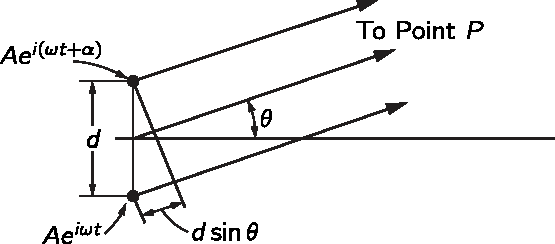
\includegraphics[width=0.9\linewidth]{fyz_fig241.pdf}
      \caption{ Dva oscilátory sestejnou amplitudou fázově posunuté o úhel \(\alpha\)
               (\cite[s.~389]{Feynman01})}
      \label{fyz:fig241}
    \end{figure}
    
    Zde jsou zahrnuty všechny případy. Zbývá nám dosadit tento výraz do (\ref{fyz:eq307}) pro 
    případ, že \(A_1 = A_2\), a můžeme vypočítat všechny výsledky pro dvě antény se stejnou 
    intenzitou.
    
    Podívejme se, co se stane v různých případech. Například důvod, proč je při \ang{30} na obr. 
    \ref{fyz:fig236} intenzita rovna \(2\), je tento: dva oscilátory jsou od sebe vzdáleny 
    \(\lambda/2\), takže při \ang{30} \(d\sin\vartheta= \lambda/4\). Proto \(\varphi_2 - \varphi_1 
    = 2\pi\lambda/4\lambda = 1/2\) a interferenční člen je roven nule. (Sčítáme dva vektory 
    svírající \ang{90;;}) Výsledkem je přepona rovnoramenného pravoúhlého trojúhelníka, rovná 
    \(\sqrt{2}\) násobené jednotkovou amplitudou. Umocníme-li ji na druhou, dostáváme intenzitu 
    dvojnásobně větší než v případě jednoho oscilátoru. Podobným způsobem lze vypočítat všechny 
    ostatní případy.
    
  \section{Příklady a cvičení}\label{fyz:IchapXXIXsecVI}

} %tikzset
%---------------------------------------------------------------------------------------------------
\printbibliography[title={Seznam literatury}, heading=subbibliography]
\addcontentsline{toc}{section}{Seznam literatury}